\documentclass[11pt,a4paper]{article}
\usepackage[T1]{fontenc}
\usepackage[utf8]{inputenc}
\usepackage{lmodern}
\usepackage[margin=27mm,headheight=15pt]{geometry}
\usepackage{microtype,amsmath,amssymb,amsthm,mathtools}
\usepackage{graphicx,xcolor,booktabs,longtable,tabularx,array}
\usepackage{enumitem,listings,fancyhdr,needspace}
\usepackage{tikz}
\usetikzlibrary{arrows.meta,positioning,fit,calc}
\usepackage{xurl}
\usepackage[colorlinks=true,linkcolor=blue!45!black,citecolor=green!35!black,urlcolor=blue!50!black]{hyperref}
\usepackage[nameinlink,noabbrev]{cleveref}
\definecolor{ink}{HTML}{172B3A}
\definecolor{accent}{HTML}{235F7B}
\definecolor{pale}{HTML}{F1F5F7}
\newcommand{\code}[1]{\texttt{\detokenize{#1}}}
\newcommand{\Lean}{Lean~4}
\newcommand{\E}{\mathcal E}
\newcommand{\G}{\mathcal G}
\newcommand{\C}{\mathcal C}
\newcommand{\R}{\mathcal R}
\newcommand{\N}{\mathbb N}
\newcommand{\synth}{\mathrel{\leadsto}}
\newcommand{\judg}[3]{#1\vdash #2:#3}
\newcommand{\File}[1]{\nolinkurl{#1}}
\newcolumntype{Y}{>{\raggedright\arraybackslash}X}
\newcolumntype{L}[1]{>{\raggedright\arraybackslash}p{#1}}
\setlist{nosep,leftmargin=1.6em}
\setlength{\parskip}{4pt}
\setlength{\parindent}{0pt}
\setcounter{tocdepth}{2}
\emergencystretch=2em
\raggedbottom
\widowpenalty=10000
\clubpenalty=10000
\displaywidowpenalty=10000
\pagestyle{fancy}
\fancyhf{}
\fancyhead[L]{\small\color{ink}Leant2: native dependent synthesis}
\fancyhead[R]{\small Architecture and algorithms}
\fancyfoot[C]{\thepage}
\lstdefinelanguage{LeanSketch}{
  morekeywords={def,theorem,example,structure,inductive,where,match,with,fun,forall,let,in,by,exact,apply,intro,cases,constructor,if,then,else,return,do,namespace,universe,termination_by,noncomputable,partial},
  sensitive=true,morecomment=[l]{--},morestring=[b]"
}
\lstset{language=LeanSketch,basicstyle=\ttfamily\small,keywordstyle=\bfseries\color{accent},commentstyle=\itshape\color{black!55},backgroundcolor=\color{pale},frame=single,rulecolor=\color{black!15},breaklines=true,columns=fullflexible,keepspaces=true,showstringspaces=false,aboveskip=8pt,belowskip=8pt,xleftmargin=3pt,xrightmargin=3pt}
\newtheorem{definition}{Definition}[section]
\newtheorem{proposition}[definition]{Proposition}
\newtheorem{theorem}[definition]{Theorem}
\newtheorem{invariant}[definition]{Invariant}
\theoremstyle{remark}
\newtheorem{remark}[definition]{Remark}
\title{\textbf{Leant2: Lean-Native Program Synthesis\\with Dependent Types and Behavioral Contracts}\\[6pt]\large Architecture, Search Algorithms, Trust Boundaries,\\and a Remotely Checked Lean Prototype}
\author{Technical design study}
\date{September 17, 2026}
\hypersetup{pdftitle={Leant2: Lean-Native Program Synthesis with Dependent Types and Behavioral Contracts},pdfauthor={Technical design study},pdfsubject={Lean-native synthesis architecture, algorithms, and checked experiments}}
\begin{document}
\maketitle
\begin{abstract}
Leant2 should not be a transcription of a Haskell synthesizer into Lean. Its central object should be an exact Lean expression under an exact local context, together with a graph of computational, logical, and operational obligations. We propose a synthesis system that combines focused dependent inhabitation, demand-directed library composition, recursion-template synthesis, and counterexample-guided behavioral refinement. All core search and reconstruction algorithms are implemented in Lean. External solvers are optional sources of proposals, never positive authority. A transactional native search state preserves universe constraints, dependent indices, local dictionaries, and correlations between holes, while immutable scoped plans make search reproducible and portable across worker restarts.

The design separates three questions that are often conflated: whether a term has the requested type, whether it satisfies the requested behavior, and whether it compiles to an acceptable executable. It also separates failed search from a proof of impossibility. Concrete algorithms are given for application-spine search, dependent constructor selection, motive generalization, checked recursive lowering, semantic pruning, scheduling, and final validation. A 133-line experimental Lean file synthesizes fourteen small declarations under Lean 4.34.0; all fourteen have empty reported axiom inventories. Additional checked examples establish the feasibility of indexed recursive definitions and verify three small logical certificates. A deliberately failing compiler test demonstrates why a separate executable-lowering stage is necessary. These experiments validate architectural mechanisms, not the performance or coverage of the proposed full system.
\end{abstract}
\vspace{5pt}
\textbf{Deliverable status.} This is a design and algorithm specification with a small checked pilot, not a completed Leant2 implementation. Listings in the article are explanatory pseudocode unless explicitly identified with a checked artifact. Source identities and validation limitations appear in Sections~\ref{sec:baseline} and~\ref{sec:experiments}.
\clearpage
\tableofcontents
\clearpage

\section{Executive design decisions}\label{sec:executive}

The recommended architecture is a \emph{native, proof-producing synthesis service}, available as a tactic, a declaration command, and a REPL operation. These entrances share one query representation and one validation pipeline. The synthesis engine owns neither the meaning of Lean types nor the truth of its answers. Lean's elaborator resolves the query; Lean's kernel checks the final declarations; an explicit policy determines which assumptions and computational features are acceptable.

The main decisions are as follows.
\begin{enumerate}
\item \textbf{Keep exact Lean types throughout search.} Use \code{Expr}, \code{Level}, native local declarations, and environment metadata. Do not rebuild a smaller type language in which term indices, proof dependencies, or universes become opaque approximations.
\item \textbf{Search over coupled obligations.} An application may create several metavariables whose types and specifications constrain one another. Backtracking must restore the entire branch and its continuation, not just the most recently selected hole.
\item \textbf{Use a portfolio, not one universal tactic.} Focused structural search handles small dependent terms; indexed library composition finds useful components; recursion templates expose inductive structure; specialized proof engines discharge logical side conditions; behavioral guidance reduces irrelevant programs.
\item \textbf{Separate semantic synthesis from executable realization.} A kernel-valid recursor term is a useful semantic model but need not be accepted by the code generator. Produce equation-oriented definitions and check their relationship to the synthesized model, or prove the contract directly for the executable definition.
\item \textbf{Make every claim carry its scope.} Type correctness, finitely many observations, a universal contract, grammar exhaustion, and mathematical impossibility are different outcomes. Neither a satisfiability-modulo-theories (SMT) solver answer nor a search timeout changes one category into another.
\end{enumerate}

A realistic first implementation should prioritize transformations of algebraic and indexed data, higher-order composition, small arithmetic witnesses, and library-backed verified functions. These are broad enough to be useful without pretending that arbitrary mathematical theorem discovery is a routine subproblem. The scope can expand through registered constructors, recursors, contracts, proof rules, and domain adapters rather than through a succession of special cases in a Haskell-to-Lean translation.

The intended advantage is not merely fewer rejected renderings. It is the ability to let \emph{Lean dependencies guide the search before a candidate exists}: an output index constrains an input witness; a proof field determines a natural number; a callback type determines a polymorphic instantiation; a recursive specification determines which accumulator must be generalized.

\section{Baseline: what should be retained, replaced, and extended}\label{sec:baseline}

\subsection{Repository identities and observed capabilities}

The repository inspection used Leant commit
\begin{center}\small\code{6bf05ad78c467989e68290f2d08bbed40802d485}\end{center}
and its Djex submodule revision
\begin{center}\small\code{e237e8667190aff38faaa590ce5b12afbffac452}.\end{center}
The Leant revision is dated September 14, 2026. Repository documentation and the source paths cited below are design evidence, not benchmarks rerun in this study. The Lean experiments use the separately identified remote environment \code{lean-4.34.0}. No claim that this is the latest available Lean release is needed.

Leant already asks Lean to elaborate queries and recheck candidates. Its fragment serializer runs on the Lean side; it is not simply a Haskell parser guessing the meaning of Lean syntax. The source explicitly retains many structural connectives and selected polymorphic applications, but treats term-indexed applications as opaque and uses bounded descriptions for recursion. This is the principal representation boundary Leant2 should remove \cite{leant-fragment}.

Djex contributes two complementary traditions: a checked propositional prover based on Dyckhoff's contraction-free intuitionistic sequent calculus (LJT), and a ranked typed-hole search engine with class evidence and resource controls. Its shared type and candidate infrastructure already enforces ownership, source association, and independent checking. Leant2 should retain those engineering principles without preserving the Haskell compatibility surface \cite{djex-architecture,djex-readme}.

Behavioral assertions are also not new to this proposal. At the inspected Leant revision, named assertions are checked against each exact candidate; successful proofs, proved negations, and inconclusive checks are distinguished. The search engines primarily produce type inhabitants before these checks. Leant2 moves behavioral constraints into partial-program search while retaining the existing refusal to identify proof failure with a counterexample \cite{leant-behavior}.

The repository's current indexing diagnostics locate a remaining difficulty in bounded composition, not simply in the absence of a primitive. A standalone handler can be found while its composition in the full context is missed. This motivates contextual component reuse and obligation-directed scheduling. It does not establish that the new design solves the original public query within its original budget \cite{leant-indexing}.

\subsection{Relationship to the existing Lean rewrite analysis}

The existing rewrite study already recommends Lean-hosted semantics, project-matched worker processes, exact source identities, and a kernel validation boundary. Those ideas are adopted rather than presented as new \cite{rewrite-study}.

There is one deliberate architectural departure. The earlier study keeps a pure neutral search representation and confines native metavariable machinery largely to preparation and lowering. Leant2 should instead use \emph{native, branch-local dependent constraints during search}. The reason is that a neutral representation restricted enough to be easy to search can recreate the very loss of dependency information that the successor is meant to remove.

This does not mean keeping a globally mutable \code{MetaM} state as the whole application. Leant2 should have two complementary representations:
\begin{quote}
An immutable, scoped \emph{search plan} records what is being constructed and how to replay it. A branch-local native \emph{constraint state} decides what the plan currently permits.
\end{quote}
The plan contains native expressions and binding structure, not an alternative approximation to Lean's type theory. It can be serialized without retaining live metavariable identifiers. The native state is disposable and can be reconstructed from a plan checkpoint.

\subsection{Scope of the rewrite}

The core, including the scheduler, indexes, search rules, behavioral adapters, proof reconstruction, and controller, is written in Lean. A Haskell installation is not required. The frontend accepts Lean syntax only. An optional solver process may be implemented in another language, just as Lean itself depends on a runtime and operating system; that process is not the semantic engine and cannot certify results.

A stronger deployment can use a small operating-system shim for process isolation or executable-identity guarantees. This is an operational option, not a justification for moving the synthesis algorithms out of Lean. A portable baseline should work without Z3, without a remote model, and without such a shim.

\section{The synthesis problem and its user-visible contract}\label{sec:query}

\subsection{An exact query}

\begin{definition}[Synthesis query]
A query is a tuple
\[
 Q=(\E,\Gamma,U,\tau,R,X,\G,\Pi,B),
\]
where $\E$ is a fixed Lean environment; $\Gamma$ is a local telescope including local definitions and instances; $U$ is its universe-parameter context; $\tau$ is the requested type; $R$ is an optional Lean proposition-valued predicate on inhabitants of $\tau$; $X$ is a collection of typed observations; $\G$ is a candidate grammar and component policy; $\Pi$ is a trust and execution policy; and $B$ is an operational budget.
\end{definition}

The elaborated query must satisfy
\[
 \E;\Gamma;U\vdash\tau:\mathrm{Sort}\,u,
 \qquad
 \E;\Gamma;U\vdash R:\tau\to\mathrm{Prop}
\]
when $R$ is present. The proposed answer is a term $t$ and, in certified-contract mode, a proof $p$:
\[
 \E;\Gamma;U\vdash t:\tau,
 \qquad
 \E;\Gamma;U\vdash p:R(t).
\]
These two declarations are the general interface. It is convenient to encode a data witness and property as a subtype in many examples, but the architecture should not assume that every query is representable by an ordinary \code{Subtype}: Lean queries can live in arbitrary sorts, including \code{Prop}. Separate term and proof fields avoid this unnecessary restriction.

The context is part of the problem. A local \code{let} must retain its value, and a local instance must retain its particular dictionary term. Universe parameters of the original declaration remain parameters; they are not free search variables to be specialized until a difficult query becomes easy.

\subsection{Three success levels, two distinct notions of failure}

\begin{center}
\begin{tabularx}{\textwidth}{@{}L{0.25\textwidth}Y@{}}
\toprule
Result & Meaning \\
\midrule
\code{TypeChecked} & The exact term inhabits the exact requested type under the audited environment. \\
\code{Observed} & The term is type checked and the listed finite observations succeeded. This is not a universal behavioral claim. \\
\code{Verified} & The term and the complete requested contract have checked proofs; the execution policy has also been evaluated and reported. \\
\code{Refuted} & A Lean proof establishes that no inhabitant satisfies the requested contract, relative to the same context and axiom policy. \\
\code{Exhausted} & The configured search space or budgeted procedure has been exhausted; the result records its grammar and incompleteness ledger. \\
\code{Unknown} & Search, proving, compilation, or a required adapter did not finish or did not support the case. \\
\bottomrule
\end{tabularx}
\end{center}

A result may be logically verified but not executable, so executability should be a separate field, such as \code{executable}, \code{noncomputableAllowed}, or \code{loweringFailed}. In an executable-only command, the last two are not successful final implementations. Keeping the logical candidate available as a diagnostic is still useful.

For refutation, the general target is
\[
 \neg\exists t:\tau,\ R(t),
\]
with $R(t)=\mathrm{True}$ for a type-only query. A term of $\tau\to\mathrm{False}$ is an equivalent concrete way to refute type inhabitation. A proof that a proposition was not derivable in a restricted intuitionistic calculus is \emph{not} a Lean proof of its negation. In particular, an intuitionistic countermodel to excluded middle cannot refute the corresponding proposition in a Lean environment allowing classical reasoning.

\subsection{Proposed entrances}

The following is surface-design notation, not implemented syntax in the pilot:
\begin{lstlisting}
def swapped (p : Prod A B) : Prod B A := by
  leant2

synth def choose : Nat -> Nat -> Nat
  satisfying fun f => forall x y,
    And (x <= f x y) (And (y <= f x y)
      (Or (f x y = x) (f x y = y)))
  using [Nat.le_decidable]
  policy executable

#synth (forall (A : Type), A -> A)
#synth? (List Nat -> List Nat) examples [(input, expected)]
\end{lstlisting}

The parser should use a reserved local identifier for the candidate in a \code{where} or \code{satisfying} clause. Unknown names in a contract are errors, not automatically introduced variables. Commands should allow an explicit component inventory, forbidden constants, an axiom profile, a proof budget, and a request for several behaviorally distinct alternatives. A missing contract should trigger an informative explanation of underdetermination, not a silent guess about the user's intended algorithm.

\subsection{Which implementations count?}

For ordinary computational synthesis, the default policy admits total, safe, pure Lean definitions that compile under the target project. It excludes newly introduced axioms, \code{sorryAx}, arbitrary choice used to obtain executable data, unproved termination, and hidden uses of the target's reference implementation. Search metaprograms themselves may use \code{partial}; that does not permit partial generated mathematical functions.

There should also be explicit proof-oriented and noncomputable modes. They may allow a documented set of standard axioms or classical constructions. An inhabitant found through choice can be perfectly legitimate mathematics without being the executable program the user requested. This distinction is a policy decision, not a contradiction in Lean's logic.

\section{Architecture and ownership}\label{sec:architecture}

\begin{figure}[ht]
\centering
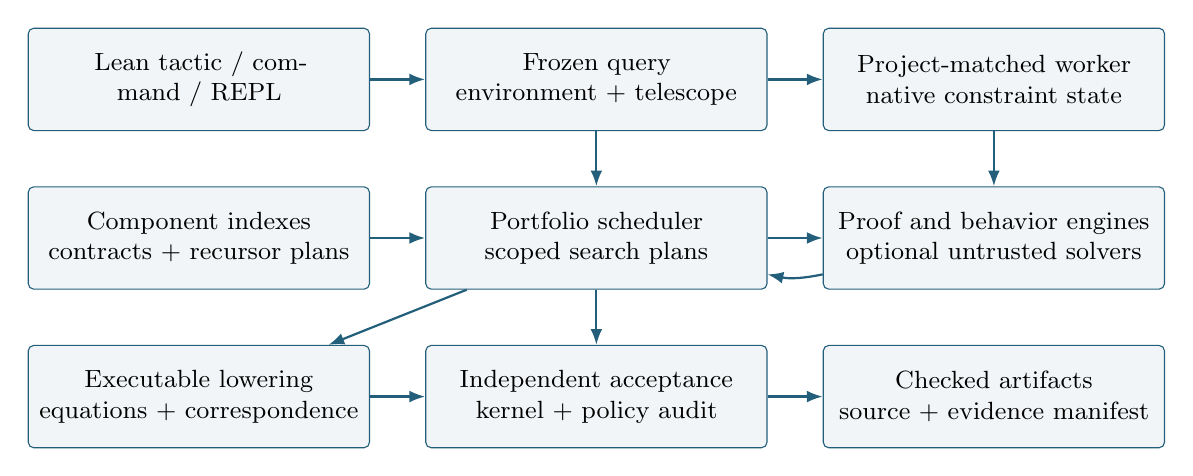
\begin{tikzpicture}[node distance=7mm and 7mm,
 box/.style={draw=accent,rounded corners=2pt,fill=pale,align=center,text width=41mm,minimum height=13mm,font=\small},
 arr/.style={-{Latex[length=2mm]},thick,draw=accent}]
\node[box] (front) {Lean tactic / command / REPL};
\node[box,right=of front] (query) {Frozen query\\environment + telescope};
\node[box,right=of query] (worker) {Project-matched worker\\native constraint state};
\node[box,below=of front] (index) {Component indexes\\contracts + recursor plans};
\node[box,below=of query] (search) {Portfolio scheduler\\scoped search plans};
\node[box,below=of worker] (logic) {Proof and behavior engines\\optional untrusted solvers};
\node[box,below=of index] (lower) {Executable lowering\\equations + correspondence};
\node[box,below=of search] (check) {Independent acceptance\\kernel + policy audit};
\node[box,below=of logic] (out) {Checked artifacts\\source + evidence manifest};
\draw[arr] (front)--(query); \draw[arr] (query)--(worker);
\draw[arr] (query)--(search); \draw[arr] (worker)--(logic);
\draw[arr] (index)--(search); \draw[arr] (search)--(logic);
\draw[arr] (logic) to[bend left=12] (search);
\draw[arr] (search)--(lower); \draw[arr] (lower)--(check);
\draw[arr] (search)--(check); \draw[arr] (check)--(out);
\end{tikzpicture}
\caption{Recommended data flow. Search and solver outputs are proposals. Only the acceptance path creates publishable results. The worker owns exact project-local Lean state; the controller need not load its compiled modules.}
\label{fig:architecture}
\end{figure}

\subsection{Module interfaces}

\begin{longtable}{@{}L{0.27\textwidth}L{0.66\textwidth}@{}}
\toprule
Module & Responsibility and boundary \\
\midrule\endhead
\code{Leant2.Frontend} & Elaborate Lean entrances; display alternatives and diagnostics. Never infer validity from printed text. \\
\code{Leant2.Query} & Freeze the goal, contract, local context, component policy, universe parameters, and authorized metavariable writes. \\
\code{Leant2.Scope} & Scope identifiers, telescope abstraction, renaming maps, dependency closure, and replay validation. \\
\code{Leant2.Search} & Portfolio scheduling, decision trails, checkpoints, continuations, alternative enumeration, and cost accounting. \\
\code{Leant2.Constraint} & Native equality attempts, delayed constraints, metavariable dependencies, instance obligations, and wake-up events. \\
\code{Leant2.Index} & Type-head and application-spine indexes, contextual component recipes, exact constant identities, and contract retrieval. \\
\code{Leant2.Recursion} & Inductive metadata, motive templates, decreasing-call capabilities, and equation-oriented output plans. \\
\code{Leant2.Behavior} & Typed samples, symbolic observations, abstract domains, counterexample-guided synthesis, and certified rejection interfaces. \\
\code{Leant2.Proof} & Bounded adapters for simplification, arithmetic, congruence, induction assistance, and optional external reconstruction. \\
\code{Leant2.Validate} & Fresh replay of exact declarations, axiom/dependency audit, compilation policy, and final evidence construction. \\
\code{Leant2.Worker} & Environment epochs, cancellation, project toolchain ownership, resource isolation, and protocol validation. \\
\bottomrule
\end{longtable}

A \code{Candidate} is intentionally an untrusted proposal. A \code{CheckedCandidate} must have a private construction path that includes final replay. This distinction prevents a plug-in or cache entry from manufacturing positive evidence merely by populating a record with plausible fields.

\subsection{Immutable plans and branch-local native state}

A conceptual node contains
\[
 S=(P,H,M,K,D,V,c),
\]
where $P$ is the partial program plan; $H$ is its obligation graph; $M$ is a native metavariable checkpoint; $K$ is the remaining continuation; $D$ is the decision trail; $V$ is the current sample/constraint version; and $c$ is accumulated cost. In an implementation, large persistent structures should be shared rather than copied wholesale.

A plan hole has a stable identifier, a scope identifier, a native target expression, and a declared role. During replay, it receives a fresh native \code{MVarId}. The stable identifier is never confused with that process-local identifier. Native expressions stored outside a live scope are abstracted over a dependency-closed telescope; they do not retain dangling free variables.

The native checkpoint includes everything a rule is allowed to change. For pure \code{MetaM} rules, this includes the metavariable context and relevant caches. A rule that invokes term or tactic elaboration must also restore the corresponding elaboration state and diagnostics. Environment-changing elaborators should be staged separately. It is not sufficient to restore a few assignments while retaining newly registered instances or simplification rules.

\begin{invariant}[Branch ownership]
Every native metavariable belongs to one query and one branch lineage. A branch can assign only its authorized search metavariables. It cannot change the frozen statement, specialize the query's universe parameters, or publish declarations into the user environment.
\end{invariant}

The public metaprogramming model already exposes local contexts, metavariables, and stateful unification; these are useful mechanisms, not an independent kernel-level proof of correct use \cite{meta-book}. The ownership invariant must be enforced around them.

\subsection{Proof-producing plug-ins}

Each plug-in declares a read/write footprint and returns one of the following conceptual results:
\begin{lstlisting}
progress     (newPlan, changedHoles, residualObligations)
solved       (termOrProof, dependencyManifest)
blocked      (watchedMetavariables, reason)
rejected     (rejectionKind, optionalCertificate)
unsupported  (feature)
interrupted  (resourceOrCancellationReason)
\end{lstlisting}

A proof adapter working on a completed candidate has no authority to change computational holes: there should be none. An integrated constraint adapter may instantiate search-owned data variables, for example by solving \code{?n = 2}, but must report those writes so that rollback and dependency wake-ups remain correct. An arbitrary tactic plug-in must never gain the ability to weaken the target simply because it runs in the same process as the search.

\section{Native dependent inhabitation}\label{sec:inhabitation}

\subsection{Judgments and focusing}

Use a bidirectional presentation of search:
\[
 \Gamma\vdash \tau\Downarrow t
 \quad\hbox{and}\quad
 \Gamma\vdash e\Uparrow\sigma.
\]
The first judgment constructs a term against an expected type. The second extends a known head expression while computing its native result type. Both carry the same branch-local constraint store; the notation suppresses it only for readability.

The first phase applies cheap, appropriate normalizations: instantiate assigned metavariables, expose the weak-head shape of the target under the configured transparency policy, and simplify obvious local definitions. Do not normalize every expression to a huge fully unfolded term. Definitions are useful abstractions, and Lean libraries contain structures whose complete expansion would destroy relevance.

For a dependent function target,
\[
 \frac{\Gamma,x:A\vdash B(x)\Downarrow t(x)}
      {\Gamma\vdash ((x:A)\to B(x))\Downarrow\lambda x.t(x)},
\]
introduce a fresh local with the original binder information. This applies equally to ordinary arguments, type arguments, propositions, and negative occurrences of polymorphic callbacks. It is a native Pi rule, not a collection of unrelated rank-specific rules.

However, an existence-preserving introduction rule need not preserve a cost optimum or every desirable source form. Eta-expanding a function may be harmless logically and undesirable operationally. Therefore the fast lane may focus eagerly, while a minimal-term mode must account for a direct existing function as an alternative.

For a structure or inductive target, constructor selection is a genuine choice. It is not an invertible proof step merely because constructors are easy to enumerate. A sum has alternative constructors; even a single-constructor dependent structure may contain a witness whose value is not determined by the type alone.

\subsection{Application-spine search}

Let a provider have native type
\[
 c:\Pi(a_1:A_1)\cdots(a_k:A_k(a_1,\ldots,a_{k-1})),\ B(\vec a).
\]
A use of $c$ begins by freshening its universe arguments and creating branch-local argument metavariables. The target constrains its result:
\[
 B(?a_1,\ldots,?a_k)\mathrel{\doteq}\tau.
\]
Every argument retains its full type, including dependence on the earlier arguments. Implicit type parameters, explicit values, and instance arguments are not stored in separate flattened lists that can lose their correlation.

The following routine describes the production algorithm.
\begin{lstlisting}
expandApplication(goal, provider, branch):
  checkpoint := saveAllRelevantState(branch)
  head := provider.withFreshUniverseMetavariables()
  for prefix in admissibleNativeSpinePrefixes(head.type):
    restore(checkpoint)
    (args, resultType, binderInfo) := openPrefix(prefix)
    outcome := tryNativeEquality(resultType, goal.target)
    if outcome is solved or legitimately postponed:
      attach goal := apply(head, args)
      register all unresolved argument and instance obligations
      record which metavariables each obligation reads
      yield childBranchWithEntireContinuation()
    else:
      record scoped failure; do not infer goal uninhabitation
\end{lstlisting}

The prefix enumeration is important. A Lean constant's useful application length can change after definitions reduce or a type variable is instantiated by a function type. A search engine must not assume that the number of syntactic leading binders in the original signature is its universal runtime or search arity. Lean's native \code{MVarId.apply} already explores argument counts and returns metavariable obligations; it is a useful first adapter, not an exhaustive higher-order application enumerator \cite{lean-apply}.

The fast lane uses native unification and demand matching aggressively. The exploration lane retains additional prefix and instantiation choices when an equality attempt is blocked or heuristic. A timeout, occurs-check complication, or failure of the elaborator's unification heuristic is not a theorem that no completion exists.

\subsection{Instantiation of polymorphic and higher-order arguments}

At an application site, first try the type parameters forced by the target and later dependent arguments. Next consider a finite, cost-ordered pool of native type expressions: local types; parameterized types already occurring in the query; provider-result types; function types suggested by demanded callbacks; and registered carrier templates. Fresh universe metavariables accompany each candidate, and the native constraints decide whether that candidate is legal.

For example, a Church fold used to implement indexing needs a function-valued carrier such as
\[
 C=\N\to\mathrm{Option}\,\alpha,
\]
not just the element type or its containing list. This carrier should arise from a demand for a residual index argument, rather than from a hard-coded rule named ``indexing.'' The pool grows with the search bound. Failure in a finite pool is a missed instantiation, not a type-theoretic impossibility.

When a callback has type
\[
 (\alpha:\mathrm{Type}\,u)\to\alpha\to\alpha,
\]
checking a candidate callback introduces the type argument as a rigid local and constructs a body uniformly in it. Conversely, applying a polymorphic provider creates fresh instantiations for that \emph{occurrence}. Reusing one occurrence's universe or dictionary assignment for a different occurrence is unsound engineering even when the printed names happen to match.

Lean's universe hierarchy must remain visible. There is no general permission to instantiate a variable ranging over \code{Type u} with every polymorphic type that would be legal in an impredicative Haskell encoding. Lean's \code{Prop} and \code{Type} have different formation and elimination behavior. A Lean-native search gains fidelity, not a license to ignore those differences \cite{lean-types}.

\subsection{Dependent constructors and indices}

Suppose a constructor is
\[
 \mathsf{cons}:\alpha\to\mathrm{Vec}\,\alpha\,n\to
                      \mathrm{Vec}\,\alpha\,(n+1).
\]
To synthesize $\mathrm{Vec}\,\alpha\,m$, applying $\mathsf{cons}$ creates the native constraint $n+1\doteq m$ and the dependent field obligations. If $m$ is definitionally a successor, this determines the predecessor. If $m$ is an expression only propositionally equal to a successor, a separate equality proof and transport may be necessary.

A structure such as
\[
 \{n:\N\mid n=2\}
\]
creates $n:\N$ and $p:n=2$. Solving $p$ by reflexivity can instantiate $n$ directly. Alternatively, a witness-first search may try $0$, discover that the continuation cannot establish $0=2$, and backtrack to other witnesses. Both strategies are legitimate. A greedy routine that commits to the first inhabitant of \code{Nat} before considering the proof field is not.

Dependent records should therefore be constructed as an obligation graph, not by a left-to-right sequence of irrevocable field completions. The production scheduler usually gives a high priority to a cheap proof field that constrains a data field. The pilot deliberately also tests witness-first exploration to expose the need for full continuation backtracking.

\subsection{Elimination, motives, and transport}

Case analysis on $x:I\,\vec p\,\vec i$ must transform the \emph{entire dependent context}, not only replace occurrences in the target's printed form. Locals whose types depend on $x$ or its indices must be reverted, generalized, or transported by Lean's elimination machinery. Use native case and recursor construction APIs; preserve the generated substitution map for each branch.

Impossible index combinations should be discharged by checked elimination or a proof using constructor disjointness/injectivity. A heuristic equality failure is not sufficient evidence that a dependent branch is unreachable. For example, matching two vectors of the same length can rule out the nil/cons combination only after the length relation is retained.

When a computation produces $v:\mathrm{Vec}\,\alpha\,(n+m)$ but the target is $\mathrm{Vec}\,\alpha\,(m+n)$, use a proof of $n+m=m+n$ and a native equality transport. Do not treat arithmetic equality as definitional equality, and do not erase the index to make the types look identical.

For caching and normalization, use scoped syntactic identities for fast keys and native checking for final reuse. For semantically justified rewriting use explicit equality certificates. Do not infer that a transitive closure of context-sensitive, metavariable-instantiating equality attempts is a valid quotient of arbitrary raw expressions. A successful conversion check under one assignment is not a reusable theorem under another.

\subsection{Type classes are computational evidence}

Instance obligations belong in the same dependency graph. An instance search may be blocked until an output parameter or a carrier type is determined; the scheduler should wake it when those dependencies change. Native instance search supplies Lean's own local and global resolution behavior, including its parameter annotations, rather than an approximate Haskell dictionary model \cite{lean-classes,lean-apply}.

There are nevertheless two distinct modes. In ordinary Lean elaboration mode, an implicit instance argument follows Lean's resolution policy. In explicitly dictionary-sensitive synthesis, supplied dictionaries may be ordinary values and the grammar may select among them. The latter must use explicit applications when necessary; it must not silently rewrite every dictionary of one type to whichever instance search chooses first.

Proof irrelevance is not data irrelevance. Two proofs of the same proposition are different from two \code{Decidable} values' computational branches or two class dictionaries with different operations. A cache that merges those dictionaries by their type can change a synthesized program's behavior.

\section{Coupled search, scheduling, and reuse}\label{sec:search}

\subsection{The correct unit of backtracking}

The unit of search is a partial program plus \emph{all} of its unfinished obligations. If a local search rule creates subgoals $H_1,\ldots,H_k$ while $K$ contains previously pending obligations, the recursive continuation is
\[
 H_1,\ldots,H_k,K,
\]
under one common substitution state. Solving $H_1$ is tentative until the continuation succeeds.

A minimal correct depth-first skeleton is:
\begin{lstlisting}
solve(obligations, state, fuel):
  remove assigned obligations
  if no obligations remain: return success(state)
  if fuel is zero: return boundedFailure
  choose one obligation h
  base := saveAllRelevantState(state)
  for refinement in orderedRefinements(h):
    restore(base)
    if refinement applies:
      r := solve(newObligations ++ remainingObligations,
                 currentState, fuel - 1)
      if r succeeds: return r
  restore(base)
  return boundedFailure
\end{lstlisting}

This is the principle implemented in the pilot. It is not a complete scheduler: a practical system should index dependencies, select constrained goals, avoid repeated failed states, and interleave branches. But replacing the single continuation with independent calls that each return their first solution loses necessary alternatives.

\subsection{Obligation graph and wake-up events}

Maintain a directed dependency relation $h\to h'$ whenever $h'$ reads a metavariable that $h$ may assign. An obligation can also be blocked on a typeclass result, a universe constraint, a proof lemma, or a previously unobserved symbolic value. Strongly connected portions are processed as coupled clusters, not topologically sorted into fictional independence.

A useful initial priority is
\[
\begin{aligned}
 \mathrm{priority}(h)&= w_1\,\mathrm{estimatedInformationGain}(h)\\
 &\quad +w_2\,\mathrm{numberOfDependents}(h)
 -w_3\,\mathrm{estimatedCost}(h).
\end{aligned}
\]
Cheap rigid equalities, index contradictions, and proof fields that determine witnesses often score well. The numerical weights are tunable heuristics. Their values do not affect the soundness of accepted terms and must not be used to certify search completeness.

After a successful assignment, increment the assignment version of affected metavariables and wake exactly the obligations whose dependencies intersect those changes. A delayed equality such as
\[
 \mathsf{recursor}(?x,\ldots)\doteq y
\]
may become decidable when $?x$ is assigned a constructor. Treating it as a permanent rigid mismatch while it is still blocked can remove valid programs.

\subsection{Fast and exploratory lanes}

The fast lane performs weighted best-first or bounded discrepancy search with strong focusing, native unification, a small type-instantiation pool, and cost-aware component retrieval. It is designed for the first useful result.

A separate exploratory lane enumerates increasingly large, explicitly described plan families. Its bounds include term constructors, binder-type complexity, universe-expression complexity, application-prefix choices, recursion schemes, and proof search fuel. Without finite bounds on these choices, ``enumerate all terms of size $n$'' can conceal an infinite alphabet of types or numerals.

The scheduler reserves a nonzero fraction of quanta for each live family, rather than allowing a promising stream to monopolize the process until it emits another candidate. A quantum bounds native reduction and proof work as well as the number of syntactic expansions. A deadline watchdog can retire a worker that does not cooperate.

The exploratory lane does not magically make a heuristic unifier complete. Its bounded completeness claims must refer to the precisely supported grammar and admissibility rules. A more ambitious certificate-enumeration lane could enumerate fully explicit candidates and proofs with increasing replay budgets, but it would be a fallback semidecision strategy, not the expected source of practical performance.

\subsection{Scope-aware component indexing}

Index global constants by native head symbol and application-spine features of their result types. Index local candidates additionally by the dependency-closed telescope they require. A solved component is stored as a recipe
\[
 (\Delta\vdash e:\sigma,\quad \text{contract lemmas},\quad \text{cost},\quad \text{provenance}),
\]
where $\Delta$ contains exactly the locals on which its type and body depend, including the dependencies of those locals.

To reuse it under $\Gamma$, find a telescope substitution $\rho:\Delta\to\Gamma$; instantiate $e$, $\sigma$, and every contract through the \emph{same} $\rho$; then native-check the resulting term against the demanded type. A name match or a matching pretty-printed type is not enough. Freshen all local and universe variables belonging to the recipe before matching.

Forward synthesis stores cheap components. Backward synthesis demands result types and proposes provider applications. A join operation connects the two: it matches demanded premises against stored components and propagates any resulting type/instance assignments across the whole application. This is particularly valuable when several possible carrier instantiations share a small handler but differ in the outer composition.

A minimal implementation uses a discrimination tree for result-type heads, a bounded map of recipes per key, and a work queue of newly derived recipes. Exact keys avoid expensive whole-environment scans; a fallback widening search prevents the initial key abstraction from becoming an undocumented completeness restriction.

\subsection{Memoization, negative caching, and semantic deduplication}

A reusable cache key includes the environment epoch or dependency manifest, scope-normalized target, contract identity, grammar policy, transparency setting, instance context, and the relevant assignments. A failure cache additionally includes the budget and reason. Failure at depth six says nothing about depth seven; a theorem-proving timeout says nothing about the truth of the proposition.

Closed, type-checked components are the safest persistent cache entries. Open components require explicit residual constraints and are substantially harder to reuse correctly. The first version should keep them within one query. Persistent storage of arbitrary native metavariable states is not recommended.

Finite observations can partition candidates into behavior buckets for ranking. They must not permanently identify all members of one bucket. Two functions agreeing on current samples may differ on the next counterexample, and in a dependent setting their output types may themselves vary with the input. Certified equivalence requires a checked equality or an explicitly sufficient relation for the contract being preserved.

\subsection{Cost and multiple answers}

Use a Pareto vector rather than a single universal notion of ``best'':
\[
 (\text{term size},\text{branches},\text{recursive structure},
   \text{dependency count},\text{proof size},\text{execution estimate}).
\]
Syntax size and estimated runtime are heuristics, not complexity theorems. A certified resource bound is a separate specification, supported by a cost semantics or a verified resource analysis. Resource-guided synthesis provides a relevant precedent, but its guarantees do not arise merely from counting AST nodes \cite{resource-synthesis}.

An answer labeled ``minimal'' needs an explicit cost model and an exhausted cheaper search prefix. Otherwise say ``lowest-cost candidate found.'' Return several alternatives when they differ in behavior, assumptions, asymptotics, or dependencies, not merely in bound-variable names.

\section{Synthesis of recursive programs}\label{sec:recursion}

\subsection{Recursors as semantic templates}

The primary recursion engine should start from the target's inductive metadata, not from an unrestricted recursive identifier. Given an inductive input, it chooses a recursor or a registered fold, constructs its motive, and creates one synthesis obligation for each constructor branch. The recursive information available in a branch is precisely the information supplied by that recursor.

For a list transformation, the branch context contains the head, the tail, and an induction-result value for the tail. For a tree, it may contain one result for each recursive child. For an indexed family, the result types carry the children's indices. This gives a finite, type-directed interface to recursion without asking the search to invent a termination proof for every arbitrary self-call.

A branch-local recursive capability records the major recursive input, permitted smaller inputs, argument dependencies, and the type of the corresponding induction result. It is not just a constant named after the function being synthesized. Any proposed recursive application must consume such a capability or discharge an explicit well-founded decrease obligation.

\subsection{Motive construction and generalization}

The central recursion problem is often the motive, not the branch body. Suppose the major input is $x:I\,\vec p\,\vec i$ and the final result type is $B(\vec i,x,\vec z)$. A useful family of motives is
\[
 M(\vec i,x)=\Pi\vec z':\Delta(\vec i,x),\ B(\vec i,x,\vec z'),
\]
where $\Delta$ generalizes selected additional inputs and any locals depending on them. The recursor supplies the varying indices and major input; $\Delta$ supplies the variables that must be permitted to change between calls.

A concrete motive-search procedure is:
\begin{lstlisting}
deriveMotivePlans(major, target, contract, context):
  read exact inductive parameters, indices, constructors, recursor
  compute locals dependent on major or its varying indices
  seed generalized locals with that dependency closure
  add ranked proposals for changing accumulators / secondary inputs
  for each bounded proposal:
    close under dependencies of the generalized locals
    abstract the result type and residual contract over the telescope
    ask Lean to check the resulting motive type
    instantiate the recursor and create constructor-branch obligations
    retain exact substitutions and recursive capabilities per branch
\end{lstlisting}

The seed does not discover every necessary invariant. Additional candidates come from user hints, the structure of recursive calls already proposed, registered accumulator patterns, and generalizations suggested by failed proof obligations. The search must be allowed to revisit the motive if a promising branch requires a changing argument not covered by the current plan.

Generalizing too little loses valid programs; generalizing too much enlarges the search and may expose irrelevant functions. The solution is a ranked, bounded family of motives with an explicit incompleteness record, not an unsupported claim that motive inference is automatic for all recursive definitions.

\subsection{Worked example: indexed mapping}

Use the family in the checked artifact:
\begin{lstlisting}
inductive Vec (A : Type u) : Nat -> Type u where
  | nil : Vec A 0
  | cons : A -> Vec A n -> Vec A (n + 1)
\end{lstlisting}
For the target
\[
 (f:\alpha\to\beta)\to\mathrm{Vec}\,\alpha\,n
                         \to\mathrm{Vec}\,\beta\,n,
\]
recursion on the vector uses the motive
\[
 M(n,xs)=\mathrm{Vec}\,\beta\,n.
\]
The nil branch has exactly the result index $0$. In the cons branch, the context contains
\[
 x:\alpha,\quad xs:\mathrm{Vec}\,\alpha\,k,
 \quad ih:\mathrm{Vec}\,\beta\,k.
\]
Constructor search reduces the result obligation to finding a $\beta$ and a vector of length $k$. Demand-directed application supplies $f(x)$, and the induction result supplies the tail. The generated equation plan is
\begin{lstlisting}
def Vec.map (f : A -> B) : Vec A n -> Vec B n
  | .nil => .nil
  | .cons x xs => .cons (f x) (Vec.map f xs)
\end{lstlisting}

This type prevents length mistakes, but it does not universally determine \emph{the intended elementwise behavior}. With richer providers, a length-preserving function can do other things. A contract is still needed when the target interface does not force the desired mapping semantics.

The supplied file contains this equation-oriented definition and its successful remote check. The pilot tactic did \emph{not} synthesize the recursive definition; it checks the representational feasibility of the planned recursion path.

\subsection{Worked example: zipping equally indexed inputs}

For
\[
 \mathrm{Vec}\,\alpha\,n\to\mathrm{Vec}\,\beta\,n
      \to\mathrm{Vec}\,(\alpha\times\beta)\,n,
\]
recurse on the first vector but generalize the second:
\[
 M(n,xs)=\mathrm{Vec}\,\beta\,n
               \to\mathrm{Vec}\,(\alpha\times\beta)\,n.
\]
The induction result in the cons branch is a function accepting \emph{any} second vector of the predecessor length. After dependent elimination of the second vector, its tail has exactly that length. The induction result can therefore be applied to the tail. Keeping the original second vector fixed would give the wrong induction interface.

This example also exercises genuine elimination of impossible index combinations. A sum-of-products approximation that forgets the common index would generate nonsensical nil/cons cases or demand defaults. Native dependent elimination removes those obligations with the appropriate evidence.

\subsection{Worked example: an accumulator invariant}

A tail-recursive list reversal uses
\begin{lstlisting}
def reverseAux : List A -> List A -> List A
  | [], acc => acc
  | x :: xs, acc => reverseAux xs (x :: acc)
\end{lstlisting}
The second argument changes, so the induction principle for correctness must quantify over it:
\[
 \forall acc,\quad \mathsf{reverseAux}(xs,acc)
                    =\mathsf{reverse}(xs)\mathbin{++}acc.
\]
In the cons branch the induction hypothesis is instantiated at $x::acc$, not at the old accumulator. The resulting list identity is discharged by the relevant append and reverse lemmas. The checked supporting theorem in the archive uses exactly this generalized route.

This suggests an effective contract-guided algorithm: when a recursive call changes an accumulator, propose a motive universally quantified over that accumulator; then synthesize a relation connecting the accumulator, the unprocessed input, and the final result. The relation can be selected from a bounded grammar of registered algebraic summaries, such as list concatenation, length, sum, or a monoid fold. Inventing arbitrary inductive invariants remains a harder tier.

\subsection{Correctness by construction for pointwise contracts}

When the result family lies in \code{Type}, a pointwise specification can be embedded in a recursive result:
\[
 F(x)=\{y:\beta(x)\mid R(x,y)\}.
\]
For a well-founded relation $\prec$, synthesizing a step
\[
 s:\Pi x,\bigl(\Pi y,\ y\prec x\to F(y)\bigr)\to F(x)
\]
and applying well-founded recursion constructs $\Pi x,F(x)$. The proof available for a recursive call is attached to a genuinely smaller argument. There is no assumption that an arbitrary recursive call already satisfies the specification.

This is an attractive internal template, but not the only representation. It can increase proof dependencies in the computational declaration. An alternative is to synthesize the recursive program and then construct a parallel induction proof using its checked defining equations. In both cases, the final candidate is accepted only after the complete proof has been checked. A global relational contract comparing multiple calls may not decompose into these pointwise subtypes at all.

\subsection{Well-founded, mutual, and nested recursion}

Beyond structurally smaller constructor fields, offer a finite family of measure templates: list length, natural-valued size, lexicographic products, and user-provided well-founded relations. For a proposed call $f(y)$ inside the definition at $x$, generate
\[
 \mu(y)<\mu(x)
\]
or the corresponding relational decrease as an explicit proof obligation. Call construction, its computational body, and its termination proof share the same plan and assumptions.

For divide-and-conquer algorithms, useful decrease lemmas should be retrieved from the library or supplied with a component contract. Testing the call on finitely many inputs cannot establish termination. A size-change analysis can rank or reject plans within a certified fragment, but does not replace Lean's final termination acceptance.

Mutually recursive definitions should be handled through a checked native mutual recursor or an explicitly constructed tagged well-founded problem. Nested and nonuniform inductive families require their actual metadata and elimination principles; flattening them into simple recursive products is not generally correct. The initial release should state which recursion plans it generates automatically while still allowing native library components of unsupported families to be used as ordinary providers.

\section{From semantic terms to executable implementations}\label{sec:lowering}

\subsection{A real compiler boundary}

A successful kernel check does not by itself imply successful executable compilation. In the remote Lean 4.34.0 experiment, the following direct custom-tree recursor definition was rejected by the code generator:
\begin{lstlisting}
def countLeaves (t : PilotTree) : Nat :=
  PilotTree.rec 1 (fun _ _ left right => left + right) t
\end{lstlisting}
The reported error identifies unsupported code generation for \code{PilotTree.rec}. A corresponding equation-oriented recursive definition compiled and evaluated successfully. This behavior is recorded as an intentional negative test in the archive, not hidden as a failed implementation attempt.

Leant2 therefore needs two linked artifacts: a semantic plan suitable for type-directed synthesis and a code-generation plan suitable for Lean's definition elaborator. This is not a second type system. Both artifacts are checked against native Lean types, and their relationship is explicit.

\subsection{Equation-oriented lowering algorithm}

For each supported recursor plan:
\begin{enumerate}
\item Recover the major argument, branch patterns, branch-local variables, recursive capabilities, and generalized arguments from the plan rather than from pretty-printed recursor text.
\item Replace each use of an induction result by a recursive call on the recorded smaller argument, supplying the actual generalized arguments at that use.
\item Produce a hygienic definition syntax tree with explicit binders, pattern equations, and, when required, a \code{termination_by} plan and decrease proofs.
\item Elaborate this definition in a staging environment containing only approved dependencies. Reject it if termination elaboration or code generation fails.
\item Prove the requested contract for the resulting executable constant. Optionally establish correspondence with the semantic model and transfer the contract through that correspondence.
\end{enumerate}

The lowering stage is allowed to change implementation structure for compilation, but cannot change the type or specification. If it introduces helper functions, those helpers form an audited dependency DAG. If source names or notation are ambiguous, emit more explicit syntax rather than trusting a successful rendering elsewhere.

For the tree experiment, a noncomputable semantic model \code{countRec} and the executable \code{countEq} satisfy the checked theorem
\[
 \forall t,\quad\mathsf{countEq}(t)=\mathsf{countRec}(t).
\]
A pointwise correspondence is enough for many pointwise contracts. An arbitrary predicate on the whole function may require a function equality and its associated extensionality principles, or a direct new proof of the predicate. The axiom policy applies to the transfer proof as well as to the original proof.

\subsection{Compilation, runtime behavior, and effects}

An executable flag means that the generated definition passed the specified compiler pipeline. It is not a machine-checked proof of the compiler's correctness, memory usage, absence of runtime failures, or asymptotic complexity. Such claims require further semantics or verified compilation infrastructure.

The synthesis grammar should exclude panic-based shortcuts, unchecked foreign implementations, and effectful evaluation unless explicitly requested. A logically convenient denotation with an aborting runtime implementation is not an acceptable ordinary implementation. Existing runtime-backed primitives are admitted only under a documented project policy, not misrepresented as newly verified by the kernel.

For monadic code, type-directed composition is useful immediately: bind, map, traversal, and local state plumbing can be synthesized from native class dictionaries. Behavioral certification should use a pure state model, weakest-precondition rules, or verified component contracts. Candidate search must not execute arbitrary \code{IO} actions to discover whether they appear to work. Partial or interactive processes need an explicit semantics and are outside the default total-function mode.

\section{Behavioral constraints inside search}\label{sec:behavior}

\subsection{Specification analysis without semantic weakening}

Retain the full elaborated $R$ as the authoritative contract. A specification analyzer may extract useful views: pointwise equalities, pre/postconditions, constructor equations, length relations, monotonicity, or invariants. Every extracted hard constraint must be accompanied by an implication showing that it is necessary for $R$, or be used only as a heuristic.

If $R$ contains a global relationship between two calls, independently assigning a postcondition to each output can lose the correlation. If $R$ contains existential quantification, replacing it by a universal input test changes the problem. The analyzer must be allowed to return ``no useful decomposition'' while complete-candidate proof search still attempts the original $R$.

A contract such as $|f(xs)|=|xs|$ does not specify reversal. Nor do length preservation and permutation together distinguish reversal from identity. Names like \code{reverse}, \code{sort}, or \code{normalize} should guide presentation and optional ranking, but cannot silently strengthen the user's formal contract.

\subsection{Typed observations}

An observation is not an untyped input/output string pair. It includes a typed substitution into the relevant input telescope, proofs that its preconditions hold, the precise output observation, and an evaluator/evidence policy. A dependent output is checked at the type induced by that particular input.

For higher-order inputs, finite tests supply concrete callback implementations or finite observations of the returned function. They cannot compare arbitrary functions for extensional equality. For open polymorphic contexts, a sample must be a legal instantiation or an existing local value; the tester cannot invent an inhabitant of an arbitrary empty type.

Observation evidence has its own strength. A native execution result is useful empirical evidence. A proof of the corresponding finite proposition is stronger. Both remain weaker than a proof of an infinite universal contract. Store that distinction in the manifest rather than giving all three outcomes the same check mark.

\subsection{Residual execution and example propagation}

Evaluate pure portions of a partial program under a legal sample until evaluation reaches a hole or an opaque operation. A residual value records the hole, its local input environment, the expected observation, and any path assumptions. It is a constraint on a \emph{particular use} of that hole, not a new global function definition.

For example, if the sketch is $g(h(x))$ and the sample requires output $y$, a known injective $g$ may induce a unique required value for $h(x)$. Without injectivity, the residual condition is relational:
\[
 \{z\mid g(z)=y\},
\]
not a guessed inverse. An operation adapter can expose a checked inverse-image rule, a finite alternatives set, or an abstract overapproximation. A stuck computation or timeout produces an unresolved observation, not a falsification.

The important implementation property is sharing: several observed calls of the same hole constrain one common synthesized function. Solving each observed call with a separate local expression would overfit the trace and fail to construct a uniform Lean term.

\subsection{A proof-aware CEGIS loop}

Counterexample-guided inductive synthesis (CEGIS) alternates candidate construction and refinement. For contracts recognized as universal pre/postconditions, use the following proof-aware loop:
\begin{lstlisting}
X := initial legal typed observations
repeat under the global budget:
  candidate := searchNativePlans(type, contractViews, X)
  if no candidate is available:
    report the precise exhausted or unknown condition
  reject obvious sample failures in the heuristic lane
  proof := tryProveCompleteContract(candidate)
  if proof succeeds and final validation succeeds:
    publish candidate with proof
  counterexample := searchForLegalCounterexample(candidate)
  if a counterexample replays and is certified:
    X := X union {counterexample}
    update residual obligations and certified rejection information
  else:
    retain candidate as unresolved; continue search or increase proof effort
\end{lstlisting}

Failure to prove $R(t)$ does not produce a counterexample. If a true candidate needs a lemma beyond the current proof budget, the system should be able to revisit it with a stronger proof plan. It should not permanently classify it as wrong.

Likewise, the absence of a counterexample from bounded testing does not prove $R(t)$. A proof can come from structural induction, existing component contracts, a reflected decision procedure, a reconstructed solver certificate, or certified exhaustive enumeration of a finite domain. The CEGIS loop itself supplies no universal verification theorem.

The loop combines the grammar/specification separation emphasized by syntax-guided synthesis with the specification-directed decomposition exemplified by refinement-type synthesis. Leant2's distinguishing engineering choice is to keep the full native dependent context authoritative while using those ideas as search guidance \cite{sygus,synquid}.

\subsection{Certified abstract pruning}

Let $C$ be a collection of possible completed programs, $I$ an input type, $O$ an output type, and $\mathrm{run}:C\to I\to O$ their mathematical interpretation. Let $\mathrm{Completion}(c)$ mean that $c$ is a legal completion of the current typed sketch. Let $P$ be a precondition and $S$ the pointwise postcondition.

An abstract analyzer can provide a predicate $A_x$ over possible outputs at a legal sample $x$, together with a proof
\[
 \forall c,\quad\mathrm{Completion}(c)\to A_x(\mathrm{run}(c,x)).
\]
An interval, length formula, constructor set, or relational symbolic expression can represent $A_x$, but its interpretation must be defined precisely.

\begin{theorem}[Safe sample-based pruning]\label{thm:pruning}
Suppose $P(x)$ holds, every legal completion has output in $A_x$, and
\[
 \forall y,\quad A_x(y)\to\neg S(x,y).
\]
Then no legal completion satisfies $\forall z,\ P(z)\to S(z,\mathrm{run}(c,z))$.
\end{theorem}
\begin{proof}
Assume $c$ is such a completion satisfying the universal contract. Soundness of the abstraction gives $A_x(\mathrm{run}(c,x))$. Exclusion gives the negation of $S(x,\mathrm{run}(c,x))$, whereas the contract and $P(x)$ give that proposition. This is a contradiction.
\end{proof}

The theorem is implemented and remotely checked as \code{safePruneAt} in \File{prototype/Certificates.lean}. It formalizes the interface an analyzer must satisfy; it does \emph{not} certify an analyzer that has not been implemented.

For a list-length example, a branch returning the empty list on a legal nonempty sample cannot satisfy a length-preservation contract. More generally, an output-length interval $[0,k]$ can refute a required length $k+1$. But an abstract ``bad output'' in an overapproximation is not automatically a concrete counterexample: the overapproximation may contain outputs no completion can produce.

\subsection{SMT and other external services}

An SMT adapter is organized as a small logical bridge, not as a parser for arbitrary Lean expressions. It declares supported source operators and sorts, a reification function, a semantic interpretation, a proof of the relevant translation direction, and a certificate-reconstruction or replay strategy.

Natural subtraction is truncated; integer subtraction is not. Division, remainder, bounded machine arithmetic, and undefined-looking library operations have concrete Lean meanings that must be matched exactly. A solver model outside the reified domain or violating a precondition is not a counterexample. Unknown and timeout responses remain unknown.

A raw \code{unsat} response can guide a heuristic lane, but cannot establish a Lean theorem. A raw \code{sat} response must be decoded into typed values and replayed against the exact candidate and contract. For certified pruning, replay must produce the required Lean evidence. Fingerprints bind a response to a query; they do not make the response true.

A useful initial set of domains is linear arithmetic over \code{Nat}/\code{Int}, constructor discrimination, list length, and small finite data. Bitvector reasoning and more complex symbolic domains should be added only with explicit evidence and axiom policies. Proof shortcuts based on native evaluation can enlarge the trusted base; the validator must inspect the actual resulting dependencies rather than infer safety from a tactic's name \cite{lean-validation}.

\subsection{Finite domains and a precise promotion rule}

When a type $I$ has a certified finite enumeration $L$, a proof for every listed input can establish a universal property. The interface is
\[
 (\forall x:I,\ x\in L)\quad\land\quad
 (\forall x:I,\ x\in L\to R(x))
 \quad\Longrightarrow\quad \forall x:I,\ R(x).
\]
The checked theorem \code{finiteValidation} is this implication. Completeness of the enumeration is essential. An arbitrary random sample list cannot be substituted for it.

For a finite function domain, equality can be checked pointwise over a certified complete input enumeration, with appropriate output equality evidence. For infinite inputs or function-valued inputs, the promotion rule does not apply merely because the current test harness has finitely many cases.

\section{Final acceptance, trust, and reproducibility}\label{sec:validation}

\subsection{Freeze the statement before searching}

The validator must receive the original elaborated query from an owner that search cannot mutate. Otherwise a search procedure can accidentally solve a specialization of the goal and claim to have solved the original. For example, assigning an external metavariable representing a supposedly arbitrary output type to the input type can turn an impossible generic map into identity.

The same problem occurs with universe parameters, unresolved coercions, hidden instance parameters, and undeclared assumptions in a specification. Preparation must either resolve them before freezing, explicitly classify them as authorized holes in the user's query, or refuse to claim a closed specification. A manifest should record the distinction between parameters and synthesis metavariables.

\Needspace{23\baselineskip}
\subsection{Acceptance pipeline}

A production acceptance routine should implement this ordered pipeline:
\begin{lstlisting}
accept(frozenQuery, proposedArtifact):
  reconstruct each scoped expression in fresh native state
  instantiate all assigned metavariables
  reject remaining expression/level metavariables or loose variables
  close the original telescope, preserving local let definitions
  rebuild approved helper declarations in dependency order
  kernel-check term against the frozen original type
  kernel-check contract proof against the original predicate at that term
  audit transitive axioms, constants, assumptions, and runtime policy
  compile the executable artifact when requested
  re-elaborate displayed source in the original presentation context
  compare its meaning and specification with the checked artifact
  return an opaque CheckedCandidate and its evidence manifest
\end{lstlisting}

The first type inference and conversion checks are cheap prechecks. Positive authority comes from checked declaration admission through the kernel, with kernel skipping disabled. The routine must not rely on an unchecked environment insertion or on a search-generated \code{inferType} success. Lean's proof-validation documentation explicitly distinguishes statement integrity, kernel checking, and environmental assumptions \cite{lean-validation}.

Local assumptions remain assumptions. If the original context contains $h:\mathrm{False}$, a synthesized inhabitant obtained from it can be perfectly valid relative to that context. The report must not present it as an unconditional construction. Likewise, imported axioms and proof shortcuts must be included in the transitive audit rather than hidden behind an imported theorem's name.

\subsection{Axiom and dependency profiles}

Useful profiles include:
\begin{description}[style=nextline,leftmargin=1.5em]
\item[Strict constructive] No axioms in the generated declaration's transitive dependency set, apart from any explicitly accepted assumptions of the query. No choice-based extraction of data and no admitted proofs.
\item[Standard proof] A configured list of standard Lean axioms is permitted in proofs and transports, with the actual list reported for each declaration. Computational behavior still has its own policy.
\item[Project-relative] Additional named project axioms may be permitted explicitly. The result is certified relative to them, not claimed axiom-free.
\end{description}

A profile should also report whether a proposition was proved by ordinary kernel-reducible reflection or by a mechanism that adds native-evaluation trust. The concrete generated dependencies, including wrappers and helper declarations, are the object of the audit. Tactic names and a reassuring command-line flag are not a substitute.

\subsection{Separate checkers and hostile plug-ins}

An in-process private constructor protects against ordinary programming mistakes, not malicious Lean metaprograms with arbitrary access to environment mutation or \code{IO}. A stronger deployment runs final checking in a separate process against the original project snapshot and a restricted serialized artifact. It does not execute arbitrary proposed tactic code as its validation protocol.

Fresh module replay and available independent checking tools can strengthen assurance. They must actually be run before their use is claimed. The experiments in this study used remote compilation and axiom reports, not an independent \code{lean4checker} run. That is sufficient evidence for the limited pilot claims but not for declaring the proposed production validator implemented.

\subsection{Environment identity and worker lifecycle}

Each committed environment receives an epoch. Query scopes, provider recipes, candidate handles, and native states are leased to that epoch and the worker that created them. Undo, import changes, worker replacement, or project changes invalidate those leases.

A long-lived Lean controller should launch the project-matched worker under the project's toolchain rather than load incompatible compiled modules into its own process. Durable state consists of source commands, component manifests, and replayable plans, not opaque pointers to native objects from a dead process. A resumed query revalidates its dependencies before continuing.

Budgeting must cover CPU work, memory, wall time, output size, recursive depth, proof work, and external process lifetime. Heartbeats are useful but do not interrupt every native or foreign operation. Cancellation must propagate rather than be caught as an ordinary failed rule. This is one of the intentional simplifications in the pilot that a production implementation must remove.

\subsection{The evidence manifest}

A final artifact should record the exact requested type and contract; original scope and universe parameters; Lean and library identities; component and forbidden-constant policies; allowed and actual axioms; the grammar and budget; execution status; proof and lowering artifacts; tested observations and their evidence strength; relevant counterexamples; and any unimplemented feature or heuristic truncation encountered.

Hashes are useful for identity and reproducibility. They are not evidence of semantic correctness. A deterministic seed and a replay plan help diagnose a failure, but a checked final term should remain independently valid even when the original heuristic ranking cannot be reproduced exactly.

\section{What can be proved about the design?}\label{sec:guarantees}

\subsection{Acceptance soundness}

\begin{proposition}[Conditional acceptance soundness]
Assume that the validator preserves the frozen statement, uses only the approved environment extensions, and successfully kernel-checks closed declarations for $t:\tau$ and $p:R(t)$. Then the accepted artifact provides Lean derivations of the original typing and contract judgments, relative to the recorded environment and assumptions. Search heuristics, solver guesses, and failed intermediate branches need not themselves be trusted for this conclusion.
\end{proposition}
\begin{proof}
The validator's first declaration supplies the typing derivation for the original $\tau$. Its second declaration supplies the derivation of the original predicate instantiated at that same term. Closing and reopening the recorded telescope restores the stated contextual judgments. Every additional assumption appears in the dependency audit by hypothesis. No unvalidated search step is used as a premise of either derivation.
\end{proof}

This is a theorem about the acceptance contract, not a proof that a particular validator implementation meets it. It also does not establish consistency of arbitrary project axioms or correctness of machine-code execution. These qualifications are essential to making the guarantee useful rather than vacuous marketing.

\subsection{Finite-fragment completeness}

\begin{proposition}[Finite search completeness under explicit assumptions]
Fix a finite grammar of scoped candidate-and-proof derivations and a finite bound. Suppose every rule is generated exhaustively, all required checks terminate and are complete for that fragment, focusing preserves the existence of an accepted derivation, and every permanent pruning step is justified. Exhaustive traversal finds an accepted derivation whenever one exists in that finite search space.
\end{proposition}
\begin{proof}
The bounded derivation tree is finite. Exhaustive traversal visits every node not pruned. A branch containing an accepted derivation cannot be removed by an existence-preserving transformation or a justified prune. Its finite sequence of terminating checks is therefore eventually performed and accepted.
\end{proof}

The hypotheses are stronger than those provided by unrestricted dependent \code{MetaM} search. In particular, native higher-order equality heuristics are not a complete decision procedure for arbitrary open constraints. Therefore the production system should claim such completeness only for separately defined and tested fragments, not for all targets accepted by the frontend.

A useful formalization order is finite first-order constructor grammars, then a simply typed functional fragment, then selected dependent index fragments with certified decidable constraints. General dependent recursion and unrestricted invariants can remain sound but incomplete extensions.

\subsection{Fairness is not completeness}

A scheduler can guarantee that each live plan family receives infinitely many quanta in an unbounded run. This ensures that a \emph{reachable finite successful path} is not starved, assuming its operations receive sufficient budgets. It does not ensure that the path is generated by an incomplete application matcher or survives heuristic pruning.

The distinction matters for reporting. A fair search that retains only the best eight components per key is still incomplete if a ninth component is needed. A proof-producing pruning rule can justify removing a branch; a beam-width setting cannot. Both may be valuable operational choices, but they belong in different parts of the evidence ledger.

\subsection{No illicit negative conclusions}

There are several legitimate negative artifacts, with different targets. A kernel-checked proof of $\tau\to\mathrm{False}$ refutes a type. A proof of $\neg\exists t:\tau,R(t)$ refutes a specification. A certified finite enumeration with checked refutations can establish that a particular grammar has no satisfying program. A classical or intuitionistic model can refute a proposition in the semantics of its explicitly stated abstraction.

By contrast, empty queues, unification failures, rejected renderings, failed proof tactics, and exhausted sample budgets are not any of these proofs. An LJT decision procedure remains useful as a fast complete solver in its own fragment, but exporting its negative results to Lean requires a theorem connecting the relevant query and semantics.

The archive includes a concrete Lean proof of
\[
 ((A\ B:\mathrm{Type})\to A\to B)\to\mathrm{False}.
\]
Instantiate a proposed function at \code{Unit} and \code{Empty}, then apply it to the unit value. This is a genuine impossible polymorphic interface. It illustrates the kind of negative certificate a public \code{Refuted} result should contain.

\section{Worked end-to-end design traces}\label{sec:traces}

\subsection{Arithmetic selection with a branch-sensitive contract}

Take $f:\N\to\N\to\N$ with contract
\[
 \forall x\,y,\quad x\le f(x,y)\ \land\ y\le f(x,y)
       \ \land\ (f(x,y)=x\ \lor\ f(x,y)=y).
\]
With a grammar containing comparison, branching, and the two inputs but excluding a ready-made maximum function, the proposed search proceeds as follows. Native introduction exposes $x$ and $y$. Observations reject constant candidates. A comparison template introduces $h:x\le y$ in one branch and its negation in the other. In the first branch, choosing $y$ makes the first inequality available as $h$, the second reflexive, and the choice disjunction immediate. In the other branch, linear order reasoning supports choosing $x$.

The program and proof obligations constrain each other: the branch assumption makes one output easy to certify. The complete contract is checked again after constructing the conditional. A test-only answer and a proof of this universal statement would have distinct result levels.

\subsection{A function-valued fold carrier for indexing}

Consider a total optional indexing operation on a list. Choose the fold carrier $C=\N\to\mathrm{Option}\,\alpha$. The base and step types become
\[
 z:C,\qquad h:\alpha\to C\to C.
\]
The intended equations determine
\[
 z(i)=\mathrm{none},\qquad
 h(x,k)(i)=
 \begin{cases}
 \mathrm{some}(x),&i=0,\\
 k(j),&i=j+1.
 \end{cases}
\]
Consequently
\[
 \mathsf{at}(xs)=\mathsf{foldr}(h,z,xs).
\]
The empty-list and head/tail equations follow directly from the fold equations; induction proves the usual optional indexing specification.

This trace suggests an actionable search strategy. Starting from a demanded result still waiting for an index argument, propose the function-valued carrier. Solve the handler once in its small telescope $(x,k,i)$. Store it as a scope-abstracted recipe. Reuse it in the outer fold through a checked telescope substitution, rather than searching for the handler again amid every outer list and index variable.

An integer-indexed interface adds a separate specification choice: negative indices may return \code{none}, use a supplied default, or mean something else. The wrapper and its proof must follow that choice. The example here is a design trace, not a claimed reproduction of the repositories' original integer-indexing acceptance case.

\subsection{A dependent witness whose first choice fails}

For $\{b:\mathrm{Bool}\mid b=\mathrm{true}\}$, a witness-first constructor search first proposes \code{false}. Its proof continuation fails. The solver restores the checkpoint containing both the witness and the proof obligation, then proposes \code{true} and closes the equality.

The pilot explicitly uses \code{ApplyNewGoals.all} so that constructor arguments can remain in original order. This tests the continuation behavior rather than relying entirely on native goal reordering to let the equality determine the witness first. The production scheduler should prefer the efficient proof-first propagation when possible, while retaining the correct fallback semantics.

\subsection{Native types beyond the initial recursive fragment}

Native representation lets the frontend preserve more than the initial solver can handle. That is an advantage only when unsupported cases remain explicit.
\begin{center}
\begin{tabularx}{\textwidth}{@{}L{0.25\textwidth}Y@{}}
\toprule
Feature & Recommended initial treatment \\
\midrule
\code{Fin}, subtypes, dependent pairs & Constructor synthesis plus arithmetic/proof obligations, fully correlated witnesses. \\
Indexed inductives & Native construction and elimination; generated recursion for supported motive plans. \\
Law-bearing structures & Synthesize fields and prove laws using registered lemmas; do not invent law proofs by testing. \\
Arrays and finite maps & Reuse verified library operations and contracts before exploring their implementation details. \\
Quotients & Use native quotient constructors/lifts and require well-definedness proofs. Do not expect inductive-constructor enumeration alone to handle them. \\
\code{Nonempty} to data & Respect elimination restrictions; computational extraction via choice requires explicit policy. \\
Function spaces and streams & Higher-order composition and pointwise reasoning; no automatic coinductive correctness claim. \\
Monadic interfaces & Native typeclass-guided composition; effectful behavior requires an explicit model. \\
\bottomrule
\end{tabularx}
\end{center}

An opaque library component remains usable if its exact type and needed contract are known. ``Cannot inspect the implementation'' should not mean ``cannot synthesize a call to it.'' Conversely, exposing the complete implementation of every dependency is rarely the right relevance strategy.

\section{Relation to existing synthesis and proof-search work}\label{sec:related}

The proposed architecture is a combination and extension of established ideas, not a claim to have invented dependent inhabitation, refinement synthesis, or counterexample-guided search.

\paragraph{Canonical.} Norman and Avigad's 2025 paper presents a Lean tactic backed by a Rust dependent-inhabitation solver, including higher-order goals, indexed recursion, and definitional equality. Its algorithm uses explicit substitutions, suspended equations, and metavariable ordering. The paper's translation omits universe levels and quotient support. Leant2 should benchmark against it, not treat dependent synthesis itself as new. The proposed difference is exact native Lean constraints, a Lean implementation, behavioral integration, executable lowering, and a production evidence boundary. The paper also motivates avoiding premature rejection when recursor reduction is blocked \cite{canonical}.

\paragraph{Aesop.} Aesop's rule-based search, normalization phases, and distinction between safer and branching rules offer an excellent model for a proof-obligation engine \cite{aesop}. Leant2 has additional responsibilities: synthesizing computational witnesses, retaining correlations between dependent fields, generating executable recursion, and satisfying user contracts. It should integrate suitable proof search rather than reimplement every prover or reduce all synthesis to invoking one tactic.

\paragraph{Refinement-type and syntax-guided synthesis.} Synquid demonstrates how rich specifications can guide recursive program construction rather than merely test finished programs \cite{synquid}. Syntax-guided synthesis makes the candidate grammar part of the problem \cite{sygus}. Leant2 adopts both lessons while retaining unrestricted native Lean specifications as the authoritative interface. Specialized decidable views accelerate search; they do not replace the source contract.

\paragraph{Djinn and Exference.} The existing dual-engine design remains valuable: complete small-fragment reasoning and heuristic program enumeration have different strengths. Leant2 should preserve the former as a certified subsolver and generalize the latter into native dependent obligation search. There is no need to preserve a Haskell frontend or its particular type-language compromises to retain those strengths.

\paragraph{What is proposed here.} The concrete design contribution is the combination of a scoped replay plan with branch-local native constraints; dependency-aware component reuse; proof-aware behavioral pruning; and a checked bridge from recursive semantic plans to executable Lean definitions. The claimed validation is limited to the artifacts in the next section. Whether this combination delivers a substantial practical coverage improvement remains an empirical question for implementation and benchmarking.

\section{Implementation sequence and acceptance gates}\label{sec:implementation}

\subsection{First vertical slice}

The smallest useful production slice has an ordinary Lean tactic entrance, a frozen query object, transactional native search, and a final checked declaration artifact. It supports local applications, Pi introduction, nonrecursive constructors and eliminations, dependent proof fields, and exact universes. It should already expose search budgets and an honest bounded-failure result.

The pilot demonstrates this direction, but production code must add exception classification, complete state ownership, assignment-difference auditing, scope-safe caches, final target replay, and resource accounting. In particular, a native \code{Expr} is a raw expression datatype, not an intrinsically typed proof that its contents are well formed. Using \code{Expr} removes lossy translations; it does not remove the need for constraints and final checking.

The initial native adapter should wrap the API operations actually exercised in the pilot: target weak-head reduction, local-context enumeration, fresh universe constants, \code{MVarId.intro1}, \code{MVarId.apply}, \code{MVarId.cases}, reflexivity, and saved-state restoration. Every wrapper has a regression test for successful use, failed use, state rollback, and interruption. This isolates Lean-version-specific details from the high-level search algorithms.

\subsection{Milestones}

\begin{longtable}{@{}L{0.12\textwidth}L{0.38\textwidth}L{0.42\textwidth}@{}}
\toprule
Stage & Delivered capability & Required gate \\
\midrule\endhead
A & Native query, scoped holes, constructive inhabitation, explicit diagnostics. & Exact target replay; multiple universes; shadowed locals; two dictionaries with different payloads; impossible and bounded-failure controls. \\
B & Dependency scheduler, indexed component retrieval, resumable portfolio, source presentation. & Coupled-witness regression; cache epoch invalidation; handler reuse in a larger context; no starvation under bounded slow rules. \\
C & Structural recursion plans, generalized motives, executable lowering. & Map, zip, accumulator reverse, and a multi-child tree fold; rejected invalid recursion; independent checks of both program and contract. \\
D & Contract decomposition, typed samples, one certified abstract domain, proof-aware CEGIS. & Necessary-condition certificates; replayed counterexamples; finite-domain promotion; adversarial spurious SMT model; inconclusive proof preserved. \\
E & Well-founded recursion, richer library contracts, optional proof/solver adapters, persistent artifacts. & Decrease proofs and axiom audit; project-version replay; resource limits; no forbidden reference implementation leakage. \\
\bottomrule
\end{longtable}

These are release gates, not time estimates. A stage can be useful before the next is finished. The behavioral layer should not wait until a huge unstructured enumerator exists: the contract representation and dependency graph belong in stage A even when only simple proof fields use them.

\subsection{Registered component contracts}

A component entry should include its exact constant and universe scheme, complete type, permitted application roles, relevant theorem names, and optional operational summaries. For example, a list-append entry can expose a length equation and a specification equation without forcing the search to unfold append recursively.

Registration must kernel-check every claimed theorem application against the exact component. User-supplied relevance tags, cost estimates, or ``commutative'' annotations are suggestions until justified. A semantic summary inferred from tests belongs to ranking metadata, not to the certified constraint database.

A contract index can begin with exact result-head matching and theorem conclusion patterns. More ambitious premise selection or learned retrieval can be added later. Regardless of how a component is retrieved, its application must pass the same native instantiation and final evidence pipeline.

\subsection{Memory and performance engineering}

The worst-case search is exponential even in small bounded grammars. Native dependency information reduces wasted branches, but does not remove combinatorial search. Engineering priorities should therefore be driven by measured expansion counts, equality-check costs, retained checkpoint memory, and proof replay time.

Share immutable expression DAGs and scope-normalized component recipes. Use small checkpoints with replay tails rather than retaining every full elaboration state forever. Compact solved proof obligations into checked expressions once their dependencies are stable. Separate cheap static index filtering from expensive native equality attempts. Cap proof-engine work per candidate so that one difficult proof cannot prevent discovery of a simpler verified implementation.

Parallel search should initially use independent workers or clearly isolated native states. A globally shared metavariable context with concurrent assignments is not a safe optimization. Share closed checked components across workers only after validating environment and scope identities. Publish results deterministically when possible, but do not confuse deterministic output order with a completeness guarantee.

\section{Experimental validation}\label{sec:experiments}

\subsection{Method and exact artifacts}

The environment available for this study had no local Lean installation and no direct container network access. The uploaded AXLE tooling described an HTTP-based checking route. Requests were sent through the available Wolfram Language evaluator using UTF-8 JSON byte arrays, with:
\begin{lstlisting}
environment      = "lean-4.34.0"
ignore_imports   = false
theorems_only    = false
content          = exact source, including checks and axiom reports
\end{lstlisting}
The service echoed the submitted source unchanged modulo trailing whitespace. The reported Lean version was 4.34.0. The main updated pilot response was not a cached response.

The exact final pilot is \File{prototype/Leant2Pilot.lean}, 133 lines including declarations, tests, and diagnostic commands. It uses \code{import Lean}, not an automatically substituted \code{import Mathlib}. Its \code{leant2_pilot} tactic searches at fuel 24 with native introduction, local application, constructor application, selected case splits, reflexivity, and full-continuation rollback.

The artifact directory also retains the first checked 128-line experiment, which used default application-goal ordering. It is historical evidence, not the final version. The final version explicitly requests all application goals in original order and adds a forced higher-rank consumer and an indexed witness.

\Needspace{27\baselineskip}
\subsection{Synthesized declarations}

\begin{longtable}{@{}L{0.28\textwidth}L{0.46\textwidth}L{0.18\textwidth}@{}}
\toprule
Declaration & Exercised mechanism & Reported axioms \\
\midrule\endhead
\code{identity} & Uniform identity over \code{Sort u}. & None \\
\code{composition} & Composition with three independent universe parameters. & None \\
\code{sCombinator} & Reuse of a local argument in higher-order application. & None \\
\code{pairSwap} & Product elimination and reconstruction. & None \\
\code{dependentApply} & Dependent function result at the selected input. & None \\
\code{dependentPair} & Sigma constructor with correlated witness and payload. & None \\
\code{higherRank} & Acceptance of a higher-rank context and uniform output. & None \\
\code{rankNConsumer} & A result obtainable by supplying a polymorphic function to a consumer. & None \\
\code{indexedWitness} & Sigma witness whose second field is \code{Fin (n + 1)}. & None \\
\code{constrainedBool} & Boolean witness coupled to an equality proof. & None \\
\code{constrainedNat} & Natural witness coupled to the proof that it equals 2. & None \\
\code{sumSwap} & Sum elimination and opposite constructor selection. & None \\
\code{modusPonens} & Proposition-valued local application. & None \\
\code{disjunctionSwap} & Proposition-valued disjunction elimination. & None \\
\bottomrule
\end{longtable}

All fourteen declarations compiled and all fourteen printed empty axiom inventories. The \code{higherRank} case alone does not prove that the polymorphic input was used: a valid solution may ignore it. The added \code{rankNConsumer} case is the stronger construction test, because an arbitrary result type is available through a consumer of a polymorphic identity-like argument. Neither test establishes exhaustive rank-N or impredicative coverage.

Seven additional examples check selected frozen types or concrete equations. The evaluated constrained natural is 2, and swapping the pair \code{(7, true)} yields \code{(true, 7)}. Two \code{fail_if_success} controls confirm bounded failure on an arbitrary map between unrelated types and on \code{False}. These are negative \emph{search controls}, not generated proofs of impossibility.

\subsection{Supporting recursive definitions and certificates}

Four supporting declarations in the pilot file were written explicitly rather than synthesized: \code{Vec.map}, \code{Vec.zip}, \code{reverseAux}, and \code{reverseAux_spec}. The first and third reported no axioms. The second and fourth reported \code{propext}. This difference is retained in the receipts and is relevant to strict versus standard proof profiles.

The separate \File{prototype/Certificates.lean} contains three small hand-written logical certificates: the concrete polymorphic noninhabitation proof, the conditional sound-pruning theorem, and the finite-enumeration promotion theorem. All three reported empty axiom inventories. It also contains a semantic tree recursor, an executable equation-oriented tree function, and their pointwise correspondence theorem. That theorem reported \code{propext}; evaluating the executable on a three-leaf tree produced 3.

These certificates prove the stated small implications and example correspondence. They do not verify the whole scheduler, the native-state adapter, a general abstract interpreter, or a general recursive-lowering compiler.

\subsection{Deliberately failing compilation probe}

\File{experiments/RecursorCompileProbe.expected-failure.lean} attempts to compile a direct custom recursor as an ordinary executable definition. The service returned \code{okay = false} and a code-generation error for \code{PilotTree.rec}. The separately checked equation-oriented version succeeds. This probe is expected to fail under the tested environment and must not be included in an undifferentiated ``all source files must compile'' build target.

The result is especially relevant to Leant2: a synthesizer that stops after finding a well-typed recursive term can still fail the user's request for an implementation. A lowering stage and explicit execution policy are therefore part of the proposed core, not a cosmetic printer improvement.

\subsection{Receipts, timings, and limitations}

\begin{center}
\begin{tabularx}{\textwidth}{@{}L{0.29\textwidth}Y@{}}
\toprule
Experiment & Remote request identity and outcome \\
\midrule
Updated pilot & \code{e8685112-e949-4837-89e6-969f4eb3682b}; compilation succeeded; no errors or failed declarations. \\
Certificates & \code{b7a9c77b-97e1-430f-a3c6-1ca890606df1}; compilation succeeded; no Lean warnings. \\
Recursor probe & \code{99ba2674-b93a-4986-8481-86859594289c}; expected code-generation rejection. \\
\bottomrule
\end{tabularx}
\end{center}

The updated pilot's response reports \code{parse_ms = 1459}, \code{total_ms = 1463}, and total request time 1586 milliseconds. These are service measurements for the whole file, including elaboration, checks, and diagnostics in a warm environment. They are not per-query synthesis benchmarks and do not demonstrate a speedup over Leant, Djex, Aesop, or Canonical.

The pilot produced unused-variable and unused-tactic linter warnings in its intentional negative controls. The service also advised using its default Mathlib import header and warned that \code{Mathlib.Tactic} was not imported. The original header was deliberately retained. No independent local toolchain replay or separate checker was available in this session. The service reports executor identities but does not supply a Mathlib commit; the archive records that limitation.

The JSON files in \File{experiments/} are clearly labeled transcriptions of selected observed response fields, not signed attestations or complete raw responses. The included reproduction client writes a full new response when run. An AXLE success flag alone is insufficient because a file containing admitted proofs may still compile; errors, failed declarations, warnings, echoed source, and axiom reports must also be inspected \cite{axle-check}.

\section{Evaluation plan for the full implementation}\label{sec:evaluation}

\subsection{Measure coverage rather than assert it}

There is no defensible measured percentage of ``practical Lean types'' in the current evidence. The fourteen synthesized examples are selected mechanism tests. A serious coverage claim requires a defined population, a reproducible sampling method, and a frozen component policy.

Build separate suites for higher-order plumbing, indexed data, structural and well-founded recursion, behavioral contracts, library-backed composition, and law-bearing structures. Keep impossible queries and adversarial controls in a separate denominator from positive synthesis tasks. Record whether each task permits direct library reuse, requires construction from primitives, or forbids a particular reference implementation.

For contracts using a known function as a specification, that reference function may appear in the proof environment but must be excluded as a computational provider in a from-scratch test. Also exclude aliases and wrappers that trivially expose it. Without this separation, apparently excellent synthesis coverage may measure only retrieval of the answer from the specification.

\subsection{Baselines and ablations}

Compare the full implementation with the pinned Leant/Djex pair, the native pilot extended only by larger budgets, a proof-search baseline where applicable, and Canonical on its overlapping supported fragment. Differences in universes, quotient support, executable output, provider availability, and contract strength must be reported rather than hidden behind one aggregate score.

Ablations should disable behavioral propagation, generalized motives, scoped component reuse, certified abstraction, and the exploratory lane one at a time. Measure not only solved tasks but also expansions, native equality attempts, proof effort, peak memory, output term size, axiom dependencies, and fresh replay time.

Fair comparisons should use the same allowed constants and source specifications when possible. Where that is impossible, report paired task subsets. A function synthesized at a more permissive universe or after adding an inhabitance assumption is not a success on the original signature.

\subsection{Adversarial regression suite}

The most valuable early regressions include a dependent witness requiring backtracking; equal-looking locals from distinct scopes; stale environment handles after undo; same-type dictionaries with different payloads; a callback requiring two distinct universe instantiations; a falsely strengthened original goal; a recursive call with no valid decrease; a compiler-rejected recursor term; a spurious solver model; an incomplete finite enumeration; and a hidden admitted proof behind a helper declaration.

Each failure must be classified correctly. A solver timeout is not a counterexample. A rejected candidate is not a refuted type. A kernel-valid noncomputable object is not an executable program. A proof depending on an unapproved axiom is not a strict constructive success.

\section{Conclusion}

Leant2 should be built around native dependent obligations rather than around a translated approximation of types. The most important change is to preserve the relationship between a program's pieces: type parameters, indices, witnesses, proof fields, callbacks, dictionaries, recursive hypotheses, and behavioral requirements all constrain one shared construction.

A practical implementation combines a fast focused lane with explicit exploratory search, reuses checked components through scoped substitutions, derives recursion plans from native inductive metadata, and lets specifications guide partial programs. A separate acceptance path protects the original statement and the user's trust policy. A separate executable-lowering path protects the difference between a mathematical term and deployable Lean code.

The checked pilot shows that a small native search can already construct several classes of terms without any Haskell type approximation. The supporting experiments also show why successful examples alone are insufficient: dependent backtracking, axiom inventories, failed code generation, and the distinction between bounded failure and refutation must all be visible. The proposed architecture makes these boundaries explicit and provides a concrete sequence for extending the prototype into a broadly useful Lean-native synthesizer.

\appendix
\section{Artifact map and reproduction}\label{app:artifacts}

\begin{center}
\begin{tabularx}{\textwidth}{@{}L{0.46\textwidth}Y@{}}
\toprule
Path & Contents \\
\midrule
\File{article/leant2.tex}, \File{article/leant2.pdf} & Self-contained article source and compiled paper. \\
\File{prototype/Leant2Pilot.lean} & Exact checked final synthesis pilot, examples, and diagnostic commands. \\
\File{prototype/Certificates.lean} & Exact checked logical certificates and the example executable-lowering correspondence. \\
\File{prototype/lean-toolchain} & Lean 4.34.0 toolchain declaration for reproduction. \\
\File{experiments/*-receipt.json} & Selected-field transcriptions of the observed checks, including their limitations. \\
\File{experiments/Leant2Pilot-first.checked.lean} & Earlier exact checked exploratory version. \\
\File{experiments/RecursorCompileProbe.expected-failure.lean} & Intentional compiler-boundary probe. \\
\File{tools/check_axle.py} & Reproduction client preserving source and saving the full service response. \\
\File{README.md}, \File{VALIDATION.md} & Usage, status, and detailed evidence distinctions. \\
\bottomrule
\end{tabularx}
\end{center}

In an environment with the pinned Lean toolchain available:
\begin{lstlisting}[language={}]
cd prototype
lean Leant2Pilot.lean
lean Certificates.lean
\end{lstlisting}
These are reproduction commands, not a claim that they were run locally in this study. For remote replay, run the client from the archive root as described in \File{README.md}. The intentional negative probe has a separate expected-failure command. To rebuild the paper, run \code{pdflatex} three times in the \File{article/} directory.

\section{Prototype boundaries to fix before production}\label{app:pilotlimits}

The pilot is intentionally compact. Its rule order is a fixed depth-first policy, not the portfolio described in this paper. Its case-split whitelist excludes general recursion. It catches rule exceptions broadly and relies on the enclosing Lean execution budget; production code must preserve cancellation and resource errors. It does not implement a private checked-result abstraction, an independent final verifier, persistent caches, library retrieval, solver protocols, or arbitrary behavioral predicates.

Its fuel is an operational bound on recursive search transitions, not a formal measure of minimal term size. Empty results are therefore bounded search failures. The initial native checks and the enclosing declaration compilation provide the positive evidence for its examples; the pilot is not itself accompanied by a proof of search completeness or an implementation-level safety theorem.

The same simplicity is useful for experimentation. It demonstrates the native API path, exact dependent applications, type-constrained witnesses, and whole-continuation rollback in a source file small enough to audit directly. Larger algorithms should preserve these properties rather than obscure them behind an unsupported claim that using Lean automatically makes every metaprogram correct.

\section{Source notes and bibliography}\label{app:sources}

Repository sources were inspected through the GitHub connector on September 17, 2026. Lean API references are pinned to v4.34.0 where an implementation path is given; online reference-manual pages may document a newer release. Research references below are primary papers or project documentation. No previously reported repository test count is presented as a new run.

\begin{thebibliography}{99}
\bibitem{leant-fragment}
V. Reshetnikov et al.
\emph{Leant: native fragment extraction}, \File{src/Leant/Synth/Fragment.hs},
revision \code{6bf05ad78c467989e68290f2d08bbed40802d485}.
\url{https://github.com/VladimirReshetnikov/Leant/blob/6bf05ad78c467989e68290f2d08bbed40802d485/src/Leant/Synth/Fragment.hs}.

\bibitem{djex-architecture}
V. Reshetnikov et al.
\emph{Djex architecture}, \File{docs/architecture.md}.
Project documentation inspected September 17, 2026; comparison dependency pinned by Leant to \code{e237e8667190aff38faaa590ce5b12afbffac452}.
\url{https://github.com/VladimirReshetnikov/Djex/blob/main/docs/architecture.md}.

\bibitem{djex-readme}
V. Reshetnikov et al.
\emph{Djex README and synthesis overview}.
\url{https://github.com/VladimirReshetnikov/Djex}.

\bibitem{leant-behavior}
V. Reshetnikov et al.
\emph{Behavioral assertions during synthesis}, \File{docs/behavioral-synthesis.md},
Leant revision \code{6bf05ad78c467989e68290f2d08bbed40802d485}.
\url{https://github.com/VladimirReshetnikov/Leant/blob/6bf05ad78c467989e68290f2d08bbed40802d485/docs/behavioral-synthesis.md}.

\bibitem{leant-indexing}
V. Reshetnikov.
\emph{Locate the remaining indexing gap in bounded composition search}.
Leant commit message, September 14, 2026.
\url{https://github.com/VladimirReshetnikov/Leant/commit/6bf05ad78c467989e68290f2d08bbed40802d485}.

\bibitem{rewrite-study}
Leant project documentation.
\emph{Rewriting Leant and Djex in Lean 4: Feasibility, Architectural Consequences, Tradeoffs, and Recommended End State}.
Study dated August 15, 2026, inspected in the September 14 repository snapshot.
\url{https://github.com/VladimirReshetnikov/Leant/blob/6bf05ad78c467989e68290f2d08bbed40802d485/docs/Leant_Djex_Lean4_Rewrite_Analysis/Leant_Djex_Lean4_Rewrite_Analysis.tex}.

\bibitem{meta-book}
Lean community contributors.
\emph{Metaprogramming in Lean 4: MetaM}.
\url{https://leanprover-community.github.io/lean4-metaprogramming-book/main/04_metam.html}.

\bibitem{lean-apply}
Lean contributors.
\emph{Native application tactic implementation},
\File{src/Lean/Meta/Tactic/Apply.lean}, v4.34.0.
\url{https://github.com/leanprover/lean4/blob/v4.34.0/src/Lean/Meta/Tactic/Apply.lean}.

\bibitem{lean-types}
Lean contributors.
\emph{The Lean Language Reference: The Type System}.
\url{https://lean-lang.org/doc/reference/latest/The-Type-System/}.

\bibitem{lean-classes}
Lean contributors.
\emph{The Lean Language Reference: Type Classes}.
\url{https://lean-lang.org/doc/reference/latest/Type-Classes/}.

\bibitem{lean-validation}
Lean contributors.
\emph{The Lean Language Reference: Validating Proofs}.
\url{https://lean-lang.org/doc/reference/latest/ValidatingProofs/}.

\bibitem{canonical}
C. Norman and J. Avigad.
\emph{Canonical for Automated Theorem Proving in Lean}.
arXiv:2504.06239, 2025. Version 1 inspected.
\url{https://arxiv.org/abs/2504.06239}.

\bibitem{aesop}
J. Limperg and A. Halkj{\ae}r From.
\emph{Aesop: White-Box Best-First Proof Search for Lean}.
Certified Programs and Proofs, 2023.
\url{https://popl23.sigplan.org/details/CPP-2023-papers/5/Aesop-White-Box-Best-First-Proof-Search-for-Lean}.

\bibitem{synquid}
N. Polikarpova, I. Kuraj, and A. Solar-Lezama.
\emph{Program Synthesis from Polymorphic Refinement Types}.
arXiv:1510.08419; PLDI 2016.
\url{https://arxiv.org/abs/1510.08419}.

\bibitem{sygus}
M. Raghothaman and A. Udupa.
\emph{Language to Specify Syntax-Guided Synthesis Problems}.
arXiv:1405.5590, 2014.
\url{https://arxiv.org/abs/1405.5590}.

\bibitem{resource-synthesis}
T. Knoth, D. Wang, N. Polikarpova, and J. Hoffmann.
\emph{Resource-Guided Program Synthesis}.
arXiv:1904.07415, 2019.
\url{https://arxiv.org/abs/1904.07415}.

\bibitem{axle-check}
Axiom Math.
\emph{AXLE Check: Lean compilation and validation endpoint documentation}.
\url{https://axle.axiommath.ai/v1/docs/tools/check/}.
Accessed September 17, 2026. Actual environment and response identities are recorded in the experiment receipts.
\end{thebibliography}
\end{document}
